\subsection{Modelo final}
Tras varias iteraciones exploratorias con distintos modelos generativos desarrollados desde cero, se optó finalmente por utilizar un modelo preentrenado que resolviera las limitaciones encontradas en cuanto a recursos y calidad de imagen: \textit{Stable Diffusion v1.4}.

\subsubsection{Motivación para el uso de modelos preentrenados}
A lo largo del proyecto, se implementaron modelos como GAN, cGAN y AttnGAN. Estas aproximaciones permitieron comprender la lógica interna de la generación de imágenes, así como los desafíos vinculados a la representación del texto y la arquitectura del generador. Sin embargo, la calidad de las imágenes generadas no era suficiente, y el coste computacional resultó demasiado elevado. Por ello, se decidió adoptar un modelo preentrenado robusto como Stable Diffusion, que ofreciera resultados inmediatos y una mayor fidelidad visual.

\subsubsection{Descripción del modelo}
Stable Diffusion es un modelo generativo basado en la técnica de difusión latente. Su funcionamiento se basa en partir de una imagen compuesta únicamente por ruido, que se refina progresivamente gracias a una red neuronal convolucional condicionada por el texto de entrada.

\subsubsection{Componentes principales}
\begin{itemize}
    \item \textbf{UNet:} red neuronal convolucional encargada del proceso de denoising, refinando la imagen en cada paso de inferencia.
    \item \textbf{Text Encoder (CLIP):} transforma la descripción textual en un espacio latente de características que orienta el proceso de generación.
    \item \textbf{Autoencoder Variacional (VAE):} codifica las imágenes reales y decodifica los resultados generados en un espacio latente comprimido.
    \item \textbf{Scheduler:} controla el nivel de ruido introducido en cada iteración de difusión, determinando la evolución temporal del proceso.
\end{itemize}

\subsubsection{Parámetros del modelo}
\begin{itemize}
    \item Resolución de entrada: \textbf{512x512 píxeles}.
    \item Pasos de inferencia: \textbf{50}.
    \item Escala de orientación: \textbf{7.5} (Guidance Scale).
    \item Tamaño del espacio latente: \textbf{64x64 píxeles}.
    \item Codificador de texto: \textbf{CLIP ViT-L/14}.
    \item Tamaño del modelo UNet: aproximadamente \textbf{860M de parámetros}.
\end{itemize}

\subsubsection{Prueba inicial de generación}
Como primer experimento de validación, se utilizó el prompt:

\begin{center}
\textit{``A beautiful landscape with mountains and a river''}
\end{center}

Se emplearon los valores por defecto del modelo y se obtuvo la siguiente imagen:

\begin{figure}[H]
    \centering
    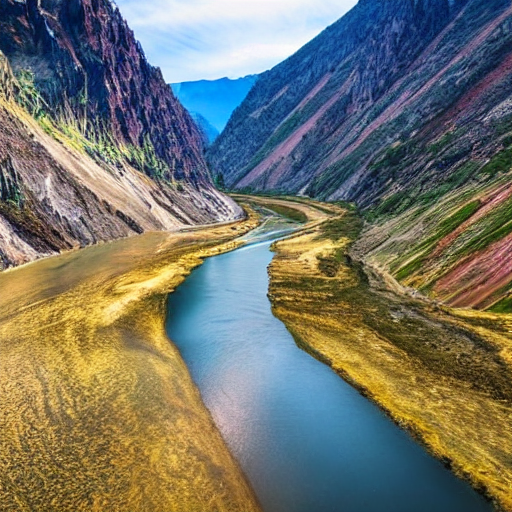
\includegraphics[width=0.4\textwidth]{original_output_image.png}
    \caption{Imagen generada con Stable Diffusion v1.4}
    \label{fig:original_image}
\end{figure}

\subsubsection{Conclusiones preliminares}
La prueba demostró que Stable Diffusion proporciona imágenes de gran calidad visual con una alta coherencia respecto a la descripción textual. Su uso supuso una mejora inmediata en términos de rendimiento y viabilidad para su integración con la plataforma Java.

\subsubsection{Optimización del modelo}
Aunque el modelo preentrenado ya ofrecía resultados prometedores, se exploraron posibles optimizaciones para mejorar aún más la precisión y adaptabilidad del sistema:

\begin{itemize}
    \item \textbf{Ajuste fino del modelo completo:} consiste en reentrenar el modelo en su totalidad utilizando un nuevo conjunto de datos, lo que permite adaptar todos sus parámetros a una tarea específica. Esta técnica mejora la especialización del modelo, aunque requiere muchos recursos computacionales y riesgo de sobreajuste si no se dispone de suficientes datos.

    \item \textbf{Modificación del espacio latente:} se centra en ajustar la estructura o dimensiones del espacio latente donde se representan las imágenes. Esto puede permitir una mayor expresividad y detalle en las imágenes generadas, así como un mejor alineamiento semántico entre el texto y la imagen.

    \item \textbf{Sustitución del decodificador VAE:} implica reemplazar el decodificador del autoencoder variacional por otro más potente o con características distintas, con el objetivo de mejorar la calidad visual de las imágenes reconstruidas desde el espacio latente.

    \item \textbf{Entrenamiento LoRA (Low-Rank Adaptation):} permite ajustar solo un pequeño subconjunto de parámetros del modelo base de forma eficiente, reduciendo el coste computacional y el riesgo de sobreajuste. Es especialmente útil cuando se quiere adaptar el modelo con recursos limitados.

    \item \textbf{Cambio en funciones de pérdida:} implica modificar la función de coste que guía el aprendizaje del modelo. Por ejemplo, se puede incorporar una pérdida perceptual o una pérdida basada en CLIP para mejorar la coherencia semántica entre la imagen y el texto.

    \item \textbf{Adaptaciones en la arquitectura UNet:} consiste en modificar la red UNet responsable del proceso de denoising durante la difusión. Esto puede incluir la incorporación de capas de atención adicionales, cambios en la profundidad de la red o en su estructura de skip connections para mejorar la capacidad del modelo.
\end{itemize}

\subsubsection{Optimización seleccionada: modificación del espacio latente}
Entre todas las alternativas exploradas, se optó por modificar el espacio latente del modelo mediante un proceso de ajuste personalizado inspirado en la técnica DreamBooth. En lugar de utilizar herramientas empaquetadas, se implementó un procedimiento propio en Python que permite especializar el modelo de difusión en nuevas clases visuales, partiendo de una colección reducida de imágenes.

Para ello, se seleccionaron 60 imágenes de tres razas concretas de perro (\textit{golden retriever}, \textit{basset hound} y \textit{whippet}) del dataset Stanford Dogs. Estas imágenes fueron preprocesadas y utilizadas en un entrenamiento supervisado en el que:

\begin{itemize}
    \item Se congelaron los módulos del codificador de texto (\texttt{CLIPTextModel}) y el decodificador (\texttt{AutoencoderKL}).
    \item Se entrenó únicamente la red \texttt{UNet2DConditionModel}, que controla la predicción del ruido en el espacio latente.
    \item Se empleó un prompt específico (\texttt{a photo of a sks dog}) como condicionamiento textual, simulando la incorporación de una nueva categoría visual.
\end{itemize}

Este entrenamiento se realizó con un tamaño de lote de 1, utilizando el optimizador AdamW y una tasa de aprendizaje reducida (\texttt{5e-6}), durante 1000 pasos. Una vez completado el entrenamiento, se generaron imágenes de prueba con prompts específicos para cada raza, como \texttt{``a photo of a sks whippet wearing sunglasses''}.

\begin{itemize}
    \item Se observó un aumento en la nitidez y realismo de las imágenes generadas.
    \item Las imágenes eran coherentes con los conceptos entrenados y semánticamente alineadas con los prompts.
    \item El coste computacional fue contenido al reutilizar componentes preentrenados y entrenar únicamente los parámetros necesarios.
\end{itemize}

Este enfoque proporciona un equilibrio óptimo entre rendimiento, especialización visual y eficiencia, y resulta especialmente útil para entornos integrados como JMR.

\begin{figure}[H]
    \centering
    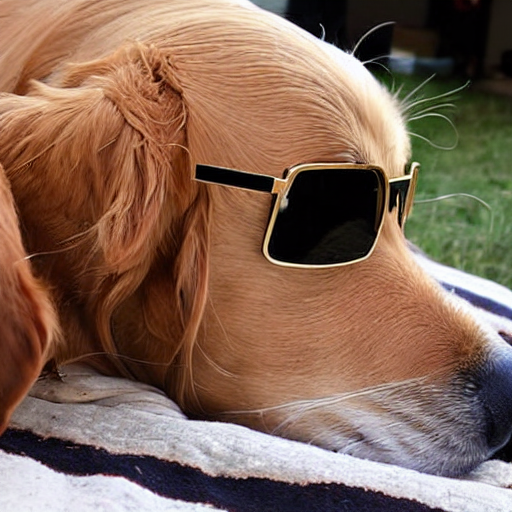
\includegraphics[width=0.45\textwidth]{golden retriever.png}
    \hfill
    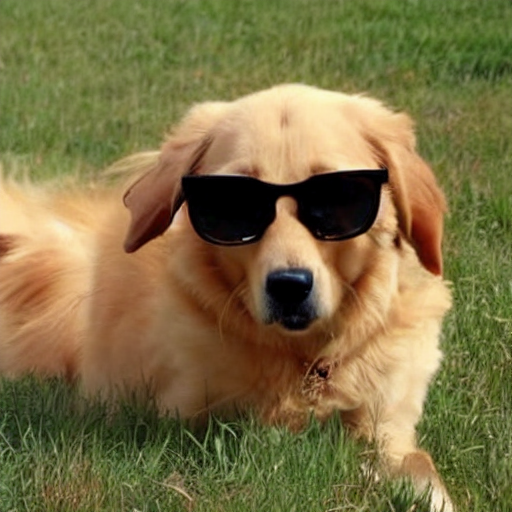
\includegraphics[width=0.45\textwidth]{golden retriever-2.png}
    \caption{Ejemplo de imágenes generadas tras la modificación del espacio latente}
    \label{fig:latent-space-optimization}
\end{figure}